 

\documentclass[12pt,a4paper]{article}

\usepackage{polski}

\usepackage{graphicx}

\usepackage{wrapfig}

\usepackage[T1]{fontenc}

\usepackage[cp1250]{inputenc}

\usepackage[top=2cm, bottom=2cm, left=3cm, right=3cm]{geometry}

\usepackage{amsrefs}

\makeatletter

\newcommand{\linia}{\rule{\linewidth}{0.4mm}}

\renewcommand{\maketitle}{\begin{titlepage}

    \vspace*{1cm}

    \begin{center}\small

    �rodowisko programisty

    \end{center}

    \vspace{3cm}

    \noindent\linia

    \begin{center}

      \LARGE \textsc{\@title}

         \end{center}

     \linia

    \vspace{0.5cm}

    \begin{flushright}

    \begin{minipage}{5cm}

    \textit{\small Autor:}\\

    \normalsize \textsc{\@author} \par

    \end{minipage}

     \end{flushright}

    \vspace*{\stretch{6}}

    \begin{center}

    \@date

    \end{center}

  \end{titlepage}%

}

\makeatother

\author{Piotr Wojtasik }

\title{Przyk�adowy dokument na laboratoria}

\begin{document}

\maketitle

\tableofcontents

\listoffigures

\newpage

\section{Tekst}

\subsection{Formatowanie tekstu}

\emph{Ten tekst jest wyr�niony}, natomiast to jest {\texttt pismo maszynowe.}

{\large W tym akapicie tekst jest nieco wi�kszy, ponadto mo�emy go np. {\bf pogrubi�}, napisa� {\it kursyw�} lub {\sc wielkimi literami.}}

\subsection{Tabele}

Przyk�adowa tabela 5 ostatnich zwyci�stw Mameda Khalidova (zawodnik MMA):
\vspace{0.5cm}
\begin{tabular}{ l | c | r }
 Bilans & Przeciwnik & Wynik \\ \hline
  21-4-2 & Yuki Sasaki & Wygrana \\ \hline
  20-4-2 & Ryuta Sakurai & Remis \\ \hline
  20-4-1 & Jorge Santiago & Przegrana \\ \hline
  20-3-1 & Jorge Santiago & Wygrana \\ \hline
  19-3-1 & Daniel Acacio & Wygrana
\end{tabular}

\section{Obrazki}

\subsection{Wy�wietlanie}

\begin{figure}[h!]
\centering
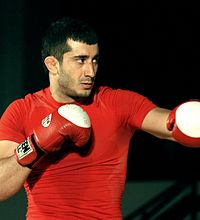
\includegraphics[bb=0 0 200 220, scale=0.5]{mamed.jpg}
\caption{Normalne zdj�cie (Mamed Khalidov)}
\end{figure}

\begin{figure}[h!]
\centering
\reflectbox{%
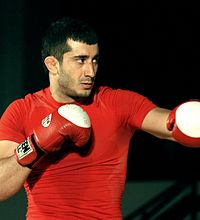
\includegraphics[bb=0 0 200 220, scale=0.5]{mamed.jpg}}
\caption{Odbicie lustrzane}
\end{figure}

\newpage

\subsection{Otoczenie tekstem}
\vspace{1cm}

\begin{wrapfigure}{r}{0.5\textwidth}
  \vspace{-6cm}
  \begin{center}
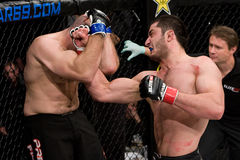
\includegraphics[bb=0 0 240 160, width=1\textwidth]{mamed2.jpg}
  \end{center}
\caption{Khalidov kontra Jason Guida}
\end{wrapfigure}
Pierwszy kontakt ze sztukami walki mia� w Groznym w wieku 12 lat trenuj�c karate. Po przyje�dzie do Olsztyna trenowa� taekwondo, zapasy i boks. W mieszanych sztukach walki startuje od 2004. Reprezentuj�c klub MMA Olsztyn zdoby� mi�dzynarodowe mistrzostwo Polski w MMA w kategoriach do 85 i 90 kg. W 2007 zwi�za� si� z organizacj� Konfrontacja Sztuk Walki.

W 2008 podpisa� kontrakt z ameryka�sk� organizacj� EliteXC na 4 walki w wadze p�ci�kiej (do 205 funt�w). 10 pa�dziernika 2008, w swoim ameryka�skim debiucie na gali ShoXC, pokona� przez techniczny nokaut Jasona Guid�. W czasie walki z�ama� palec u prawej r�ki. Kolejne wyst�py w Ameryce nie dosz�y do skutku z powodu zawieszenia dzia�alno�ci przez EliteXC z powod�w finansowych.\\

\newpage

\section{Matematyka}
\vspace{1cm}

\begin{center}
Uk�ad r�wna�:
\vspace{1cm}
$$\left\{\begin{array}{rcl}
a&=&b+c\\
b&=&2a\\
c&=&-\pi
\end{array} \right.$$
\vspace{1cm}

Macierz:
\vspace{1cm}
$$\left[\begin{array}{ccc}
2+\lambda&1&3\\
3&-6+\lambda&5\\
9&-2&-3+\lambda
\end{array}\right]$$
\vspace{1cm}

Definicja funkcji:
\vspace{1cm}
$$f(x)=\left\{
\begin{array}{ccc}
\sin{x}&\mbox{dla}&x<0\\
0&\mbox{dla}&x=0\\
\cos{x}&\mbox{dla}&x>0
\end{array}
\right.$$
\end{center}

\newpage

\section{Bibliografia}
\vspace{3cm}
\begin{bibdiv}
\begin{biblist}

\bib{http://en.wikibooks.org/wiki/LaTeX/}{article}{
    author={Wikipedia},
     title={Creative Commons Attribution-ShareAlike License},
   address={World},
      date={2005},
}
\url{http://en.wikibooks.org/wiki/LaTeX/},

\bib{http://sinatra.inf.ug.edu.pl/}{article}{
    author={W�odzimierz Bzyl},
     title={�rodowisko programisty},
      date={2008},
}
\url{http://sinatra.inf.ug.edu.pl/~wbzyl/},

\bib{http://pl.wikipedia.org/wiki/Mamed_Khalidov}{article}{
    author={Wikipedia},
     title={Mamed Khalidov},
      date={2010},
}
\url{http://pl.wikipedia.org/wiki/Mamed_Khalidov},

\end{biblist}
\end{bibdiv}
\end{document}
